\documentclass[12pt,twoside]{report}

%%%%%%%%%%%%%%%%%%%%%%%%%%%%%%%%%%%%%%%%%%%%%%%%%%%%%%%%%%%%%%%%%%%%%%%%%%%%%

% Definitions for the title page
% Edit these to provide the correct information
% e.g. \newcommand{\reportauthor}{Timothy Kimber}

\newcommand{\reporttitle}{Java Algorithms for Computer Performance Analysis}
\newcommand{\reportauthor}{Ong Wai Hong}
\newcommand{\supervisor}{Dr. Giuliano Casale}
\newcommand{\degreetype}{Master of Research}

%%%%%%%%%%%%%%%%%%%%%%%%%%%%%%%%%%%%%%%%%%%%%%%%%%%%%%%%%%%%%%%%%%%%%%%%%%%%%

% load some definitions and default packages
%%%%%%%%%%%%%%%%%%%%%%%%%%%%%%%%%%%%%%%%%
% University Assignment Title Page 
% LaTeX Template
% Version 1.0 (27/12/12)
%
% This template has been downloaded from:
% http://www.LaTeXTemplates.com
%
% Original author:
% WikiBooks (http://en.wikibooks.org/wiki/LaTeX/Title_Creation)
%
% License:
% CC BY-NC-SA 3.0 (http://creativecommons.org/licenses/by-nc-sa/3.0/)
% 
%
%%%%%%%%%%%%%%%%%%%%%%%%%%%%%%%%%%%%%%%%%
%----------------------------------------------------------------------------------------
%	PACKAGES AND OTHER DOCUMENT CONFIGURATIONS
%----------------------------------------------------------------------------------------
\usepackage[a4paper,hmargin=2.8cm,vmargin=2.0cm,includeheadfoot]{geometry}
\usepackage{textpos}
\usepackage{natbib} % for bibliography
\usepackage{tabularx,longtable,multirow,subfigure,caption}%hangcaption
\usepackage{fncylab} %formatting of labels
\usepackage{fancyhdr} % page layout
\usepackage{url} % URLs
\usepackage[english]{babel}
\usepackage{amsmath}
\usepackage{graphicx}
\usepackage{dsfont}
\usepackage{epstopdf} % automatically replace .eps with .pdf in graphics
\usepackage{backref} % needed for citations
\usepackage{array}
\usepackage{latexsym}
\usepackage[toc,page]{appendix}
\usepackage[pdftex,pagebackref,hypertexnames=false,colorlinks]{hyperref} % provide links in pdf

\hypersetup{pdftitle={},
  pdfsubject={}, 
  pdfauthor={},
  pdfkeywords={}, 
  pdfstartview=FitH,
  pdfpagemode={UseOutlines},% None, FullScreen, UseOutlines
  bookmarksnumbered=true, bookmarksopen=true, colorlinks,
    citecolor=black,%
    filecolor=black,%
    linkcolor=black,%
    urlcolor=black}

\usepackage[all]{hypcap}

\usepackage{amsthm}
%\usepackage{color}
%\usepackage[tight,ugly]{units}
%\usepackage{float}
\usepackage{empheq}
\usepackage[most]{tcolorbox}
%\usepackage[colorinlistoftodos]{todonotes}
%\usepackage{ntheorem}
% \theoremstyle{break}
\newtheorem{theorem}{Theorem}[section]
\newtheorem{corollary}{Corollary}[theorem]
\newtheorem{lemma}[theorem]{Lemma}
% \newtheorem{remark}{Remark}
%\newtheorem{proof}{Proof}
\newtheorem{definition}{Definition}[section]
\usepackage{amssymb} % for special math symbols
\usepackage{booktabs} % for special tables
\usepackage{float} % for fixed tables/figures
\usepackage{enumitem}
\usepackage{listings}
\usepackage{color}

%%% Default fonts
\renewcommand*{\rmdefault}{bch}
\renewcommand*{\ttdefault}{cmtt}



%%% Default settings (page layout)
\setlength{\parindent}{0em}  % indentation of paragraph

\setlength{\headheight}{14.5pt}
\pagestyle{fancy}
\renewcommand{\chaptermark}[1]{\markboth{\chaptername\ \thechapter.\ #1}{}} 

\fancyfoot[ER,OL]{\sffamily\textbf{\thepage}}%Page no. in the left on odd pages and on right on even pages
\fancyfoot[OC,EC]{\sffamily }
\renewcommand{\headrulewidth}{0.1pt}
\renewcommand{\footrulewidth}{0.1pt}
\captionsetup{margin=10pt,font=small,labelfont=bf}

%--- chapter heading

\def\@makechapterhead#1{%
  \vspace*{10\p@}%
  {\parindent \z@ \raggedright \sffamily
    \interlinepenalty\@M
    \Huge\bfseries \thechapter \space\space #1\par\nobreak
    \vskip 30\p@
  }}

%---chapter heading for \chapter*  
\def\@makeschapterhead#1{%
  \vspace*{10\p@}%
  {\parindent \z@ \raggedright
    \sffamily
    \interlinepenalty\@M
    \Huge \bfseries  #1\par\nobreak
    \vskip 30\p@
  }}
  
% -- Java code listing

\definecolor{dkgreen}{rgb}{0,0.6,0}
\definecolor{gray}{rgb}{0.5,0.5,0.5}
\definecolor{mauve}{rgb}{0.58,0,0.82}

\lstset{frame=tb,
  language=Java,
  aboveskip=3mm,
  belowskip=3mm,
  showstringspaces=false,
  columns=flexible,
  basicstyle={\small\ttfamily},
  numbers=none,
  numberstyle=\tiny\color{gray},
  keywordstyle=\color{blue},
  commentstyle=\color{dkgreen},
  stringstyle=\color{mauve},
  breaklines=true,
  breakatwhitespace=true,
  tabsize=3
}

% --- pretty math box

\newtcbox{\mymath}[1][]{%
    nobeforeafter, math upper, tcbox raise base,
    enhanced, colframe=gray,
    colback=blue!60!green!10, boxrule=1pt,
    #1}

\newtcbox{\mymathtwo}[1][]{%
    nobeforeafter, math upper, tcbox raise base,
    enhanced, colframe=black,
    colback=white, boxrule=.5pt,
    #1}

\allowdisplaybreaks

% load some macros
% Here, you can define your own macros. Some examples are given below.

\newcommand{\R}[0]{\mathds{R}} % real numbers
\newcommand{\Z}[0]{\mathds{Z}} % integers
\newcommand{\N}[0]{\mathds{N}} % natural numbers
\newcommand{\C}[0]{\mathds{C}} % complex numbers
\renewcommand{\vec}[1]{{\boldsymbol{{#1}}}} % vector
\newcommand{\mat}[1]{{\boldsymbol{{#1}}}} % matrix


\date{August 2018}

\begin{document}

% load title page
% Last modification: 2015-08-17 (Marc Deisenroth)
\begin{titlepage}

\newcommand{\HRule}{\rule{\linewidth}{0.5mm}} % Defines a new command for the horizontal lines, change thickness here


%----------------------------------------------------------------------------------------
%	LOGO SECTION
%----------------------------------------------------------------------------------------


\includegraphics[width = 4cm]{./figures/imperial}\\[0.5cm] 

\center % Center remainder of the page

%----------------------------------------------------------------------------------------
%	HEADING SECTIONS
%----------------------------------------------------------------------------------------

\textsc{\Large Imperial College London}\\[0.5cm] 
\textsc{\large Department of Computing}\\[0.5cm] 

%----------------------------------------------------------------------------------------
%	TITLE SECTION
%----------------------------------------------------------------------------------------

\HRule \\[0.4cm]
{ \huge \bfseries \reporttitle}\\ % Title of your document
\HRule \\[1.5cm]
 
%----------------------------------------------------------------------------------------
%	AUTHOR SECTION
%----------------------------------------------------------------------------------------

\begin{minipage}{0.4\textwidth}
\begin{flushleft} \large
\emph{Author:}\\
\reportauthor % Your name
\end{flushleft}
\end{minipage}
~
\begin{minipage}{0.4\textwidth}
\begin{flushright} \large
\emph{Supervisor:} \\
\supervisor % Supervisor's Name
\end{flushright}
\end{minipage}\\[4cm]


%----------------------------------------------------------------------------------------
%	FOOTER & DATE SECTION
%----------------------------------------------------------------------------------------
\vfill % Fill the rest of the page with whitespace
Submitted in partial fulfillment of the requirements for the MSc degree in
\degreetype~of Imperial College London\\[0.5cm]

\makeatletter
\@date 
\makeatother


\end{titlepage}



% page numbering etc.
\pagenumbering{roman}
\clearpage{\pagestyle{empty}\cleardoublepage}
\setcounter{page}{1}
\pagestyle{fancy}

%%%%%%%%%%%%%%%%%%%%%%%%%%%%%%%%%%%%
\begin{abstract}
    Queueing network theory is an important probabilistic analytical modelling tool for computer performance analysis, when designing and optimizing computer systems. A number of exact methods exist for the calculation of performance measures and state probability normalizing constants. The latter quantity is important as it appears in likelihood functions for the inference of queueing network models based on measurement data. These exact algorithms include the Convolution algorithm, RECAL, and MoM algorithms. While these provide exact answers, they generally do not scale well with the number of stations, customer classes and customer populations in the model.
    \\\\
    A new integral form of the normalizing constant, which takes the form of an integral on the simplex is proposed. Through the logistic (or log-ratio) transform, Laplace's method could be applied to compute this quantity. Laplace's method's applicability to this problem indicates the suitability of Importance Sampling on the integration domain, centered around the integrand's stationary point.
    \\\\
    This project focuses on the implementation of the Logistic Sampling algorithm as it was initially proposed, in Java. This involved a thorough understanding of the proofs and methods that make this computation possible. Novel contributions to this project include several new results concerning different transform types. Besides that, this project was able to see the derivation of results for, and implementation of an extended Logistic Sampling algorithm that catered for multi-server models.
\end{abstract}

\cleardoublepage
%%%%%%%%%%%%%%%%%%%%%%%%%%%%%%%%%%%%
\section*{Acknowledgments}
I wish to thank my supervisor, Dr. Giuliano Casale for his patience and enthusiasm in guiding me through this project.
\\\\
I also wish to thank my family for their financial and emotional support throughout this course

\clearpage{\pagestyle{empty}\cleardoublepage}

%%%%%%%%%%%%%%%%%%%%%%%%%%%%%%%%%%%%
%--- table of contents
\fancyhead[RE,LO]{\sffamily {Table of Contents}}
\tableofcontents 


\clearpage{\pagestyle{empty}\cleardoublepage}
\pagenumbering{arabic}
\setcounter{page}{1}
\fancyhead[LE,RO]{\slshape \rightmark}
\fancyhead[LO,RE]{\slshape \leftmark}

%%%%%%%%%%%%%%%%%%%%%%%%%%%%%%%%%%%%
\chapter{Introduction}

\begin{figure}[tb]
\centering

\includegraphics[width = 0.4\hsize]{./figures/imperial}
\caption{Imperial College Logo. It's nice blue, and the font is quite stylish. But you can choose a different one if you don't like it.}
\label{fig:logo}
\end{figure}

Figure~\ref{fig:logo} is an example of a figure. 

%%%%%%%%%%%%%%%%%%%%%%%%%%%%%%%%%%%%
\chapter{Background}

The aim of this chapter is to provide a theoretical background to the reader based on the ideas behind queueing theory, which forms the basis of the work done in this project. Besides that it also aims to provide context regarding the specific problems this project wishes to address with respect to queueing networks and its properties of interest.
\\\\
The summary of this chapter is as follows: section \ref{sec:intro_to_markov} aims to provide important definitions and the basic mathematical theory of Markov chains which underlies the field of queueing theory and queueing networks. Sections \ref{sec:QueueingSystems} and \ref{sec:QNetworks} introduce the idea of service centres, queues, and queueing networks, focusing on Markovian queues which are of primary interest in this project. Finally, section \ref{sec:AlgorithmsPFQN} introduces what is called the product-form solution of queueing networks, which is an important result that enables the formulation of efficient algorithms for the analysis and evaluation of queueing networks.

\section{Introduction to Markov Chains}\label{sec:intro_to_markov}

In this section we provide the definitions necessary to define Markov Processes, and Markov Chains, with special attention paid to Continuous-Time Markov Chains (CTMC's). This section assumes knowledge of stochastic processes.

\begin{definition}
    % Def 2.3
    A stochastic process \(\{X_t : t \in T\}\) constitutes a Markov process, if \(\forall t = t_0 < t_1 < ... < t_n\) and all \(s_i \in S\) it satisfies the Markov property:
    \begin{equation}\label{eq:MarkovProperty}
        P(X_{t_{n+1}}=s_{n+1} | X_{t_n} = s_n, X_{t_{n-1}}=s_{n-1}, ... , X_{t_0}=s_0) = P(X_{t_{n+1}}=s_{n+1} | X_{t_n} = s_n)
    \end{equation}
\end{definition}

The Markov property essentially states that the conditional PDF of \(X_{t_{n+1}}\) depends only on the last previous value of \(X_{t_n}\) and not not the earlier values before \(X_{t_n}\). 
\\\\
The concept of time-homogeneity is stated as the following:

\begin{definition}
    A Markov process is time-homogeneous if the following holds for the PDF of a random variable of a stochastic process at time \(t\), \(X_{t}\):
    \begin{equation}\label{eq:TimeHomogeneity}
        P(X_{t + \tau}=s_{i} | X_{t}=s_{j}) = P(X_{\tau}=s_{i} | X_{0}=s_{j})
    \end{equation}
\end{definition}

This property essentially states that the conditional PDF of \(X_{t+\tau}=s_{i}\) on the states given the state at \(X_{t}=s_{j}\) does not depend on the value of the time instant \(t\), but only on the elapsed time \(\tau\). Time homogeneity implies the memoryless property for state holding times, or state sojourn times.

\begin{definition}
    A discrete time Markov chain (DTMC) governs a discrete time (as opposed to continuous time) stochastic process, if the process has a countable state space \(S\), and satisfies the following relations on the conditional PMF, given \(n+1\) consecutive discrete time points of observation:
    \[P(X_{n+1} | X_n=s_n , X_{n-1}=s_{n-1} , ... , X_0=s_0 ) = P(X_{n+1} | X_n=s_n)\]
    This is Markov property re-stated in discrete time, for a discrete state space. 
\end{definition}

A DTMC is characterized by the state transition matrix \(\mathbf{P}\), where \(p_{ij}\) is the state transition matrix, giving a probability to transition from state \(s_i\) to state \(s_j\) at the next time instant, given that the current state of the discrete-time Markov process is \(s_j\). A time-homogeneous DTMC has a fixed state transition matrix.
\\\\
Several other desirable properties for a DTMC to have include \textit{irreducibility}, consisting only of \textit{positive recurrent states}, and is \textit{aperiodic}. The reader is advised to consult \cite{Bolch2006QueueingApplications} for details. The above properties all belong to what is called an \textit{ergodic} DTMC, and implies that a unique steady-state probability vector \(\mathbf{\pi}\) for the DTMC exists. This is given by the solution to the equation:
\begin{equation}
    \boldsymbol{\pi} = \mathbf{P}\boldsymbol{\pi}
\end{equation}

\begin{definition}
    A Continuous time Markov Chain (CTMC) governs a stochastic process, if the stochastic process satisfies the Markov property (\ref{eq:MarkovProperty}) for a countable state space \(S\). It is time homogeneous if it satisfies (\ref{eq:TimeHomogeneity}). 
\end{definition}
Given state transition probabilities \(p_{ij}(u,v)\) between times \(u\) and \(v\), and the unconditional state probabilities \(p_i(u)\), \(p_j(v)\). The following equation holds by the law of total probability:
\begin{equation}
    p_j(v) = \sum_{i \in S} p_{ij}(u,v) p_i(u)
\end{equation}
In the time-homogeneous case, this becomes:
\begin{equation}\label{eq:time_homo_unconditional_probs}
    p_j(t) = \sum_{i \in S} p_{ij}(0,t) p_i(0)
\end{equation}

The \textit{Chapman-Kolmogorov} equations are given, for a CTMC:
\begin{equation}\label{eq:CK_eqns}
    p_{ij}(u,v) = \sum_{k \in S} p_{ik}(u,w)p_{kj}(w,v)
\end{equation}
We can also define instantaneous transition rates \(q_{ij}(t)\) of a CTMC, and this is defined:
\begin{equation}\label{eq:transition_rates}
\begin{split}
    q_{ij}(t) & = \lim_{\Delta t \rightarrow 0} \frac{p_{ij}(t,t + \Delta t)}{\Delta t}, \quad i \neq j \\
    q_{ii}(t) & = \lim_{\Delta t \rightarrow 0} \frac{p_{ii}(t,t + \Delta t) - 1}{\Delta t} = -\sum_{j \neq i} q_{ij}(t)
\end{split}
\end{equation}

Without going into too much detailed derivations, the equations (\ref{eq:CK_eqns}) and (\ref{eq:transition_rates}) gives us the time-homogeneous version of the Kolmogorov forward equations:
\begin{equation}
    \frac{d p_{ij}(t)}{dt}  = \sum_{k \in S} p_{ik}(t)q_{kj}
\end{equation}
Where the time-independent transition rates \(q_{kj}\) is used. Combining this with (\ref{eq:time_homo_unconditional_probs}) gives us :
\begin{equation}
    \frac{d p_j (t)}{dt} = \sum_{i \in S} q_{ij} p_i(t)
\end{equation}

The time-homogeneity property and memorylessness property implies that the state holding time for a state \(s_i\) in a CTMC is exponentially distributed, and that the the probability of a transition \(p_{ij}\) in any given time interval \(\Delta t\) is Poisson-distributed:
\[p_{ij}(N=n) = \frac{(r \Delta t)^n exp(-r \Delta t)}{n!}\]

For an \textit{ergodic} CTMC, the steady-state distribution of \(p_j\) exists. By setting \(\frac{dp_i(t)}{dt} = 0\), this gives us what is known as the global balance equations:
\begin{equation}\label{eq:global_balance_equations}
  -p_i(t) \sum _ {j \in S, j \neq i}q_{ij} + \sum_{j\in S, j \neq i} p_j(t)q_{ji} = 0  
\end{equation}

Or in matrix form:
\[\mathbf{pQ=0}\]
Where \(\mathbf{Q}\) is a matrix where the off-diagonals elements are the inter-state transition rates, \(q_{ij}\), and the diagonal elements is the negative sum of the entire row: \(q_{ii} = -\sum _ {j \in S, j \neq i}q_{ij}\). In order to solve for \(\mathbf{p}\), one must introduce the normalizing condition \(\sum_i p_i = 1\) into the GBE's, so that \(\mathbf{Q}\) becomes non-singular.
\\\\
CTMC's governing Poisson processes form the basis of mathematical analysis for what are known as Markovian queues, which will be introduced in the next section.

\section{Queueing Systems}\label{sec:QueueingSystems}

In this section, we aim to describe queueing systems in practice, using ideas regarding the solution of CTMC's derived in the previous section.
\\\\
Queueing systems provide a means of evaluating the performance of congestion systems. These are systems that provide a finite resource or capacity to jobs or customers that can demand them. These systems can include networks of computer systems, tele-communication networks, manufacturing systems and others. The field of queueing theory is concerned with predicting system performance under different conditions, in order to assist with tasks such as capacity planning and system parametrization. Performance indices such as system utilization, system throughput, response times are of great interest. 
\\\\
A service centre, in the context of queueing theory, is characterized using the following:
\begin{itemize}[noitemsep]
    \item The arrival process of customers or jobs into the service centre
    \item The customer/job service process
    \item The size of the queue (for waiting jobs). In this project, we restrict ourselves to infinte queue length service centres only.
    \item The scheduling algorithm of job completion
    \item The number of parallel job processing units in the service centre
\end{itemize}

For convenience, the term 'queue', 'node', and  'service centre' will be used interchangeably in this project. 
\\\\
Kendall's notation describes a queueing system using the following notation : \(A/S/c\). \(A\) denotes the arrival process of jobs/customers into the queue, \(S\) denotes the service process, and \(c\) gives the number of parallel processing units/servers in the queue. In this project, we will be using the notation \(A/S/c-D\) where \(D\) denotes the scheduling discipline of the queue.
\\\\
\(S/A=M\) means that the arrival/service process is Markovian, and can be described as a memoryless Markov Process, or a Poisson process. The times between arrival/service events are thus described by an exponential distribution. On the other hand, \(S/A=G\) means that these processes are described by a \textit{general} distribution, which can sometimes be modelled using a Markov process (e.g. Erlang-j distributed) \cite{BalsamoProductNetworks}. In this project we focus only on the case where \(S=A=M\). 
\\\\
Scheduling disciplines include but are not restricted to the following:
\begin{itemize}[noitemsep]
    \item \textbf{FCFS} : The first-come-first-serve scheduling discipline always services the first job in the queue.
    \item \textbf{PS}: Processor sharing. All jobs in the queue share resources equally.
    \item \textbf{LCFS}: Last-come-first-serve. The last job in the queue is served first, at all times.
\end{itemize}
However, in the context of this project, we will mostly be considering the above cases.

\subsection{M/M/1 queuing system} \label{sec:MM1Qsystem}
The simplest queuing system possible is the M/M/1 first-come-first-serve (FCFS) system. This system has an exponential arrival rate \(\lambda\), and a service rate \(\mu\).

\begin{figure}[H]
\begin{center}
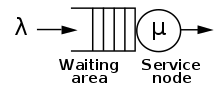
\includegraphics[width=0.4\textwidth]{Chap2_AlgorithmsPFQN/MM1_diagram.png}
\caption{Schematic of an M/M/1 queue}
\label{fig:MM1_schematic}
\end{center}
\end{figure}

The state of such a system can be uniquely defined by its population (or queue length). Assuming the service time distribution, and the arrival times are memoryless, the system can be modelled by a birth-death Markov process. The CTMC representing this is shown in figure \ref{fig:MM1_BDP}. For an open M/M/1 system with the arrival and service rates given above, several important results could be obtained. Firstly, the steady-state probabilities can be obtained by solving the global balance equations (\ref{eq:global_balance_equations}), which is uniquely described by the following set of equations:
\[ \lambda p_0 = \mu p_1\]
\[ (\lambda + \mu) p_0 = \lambda p_{n-1} + \mu p_{n+1}\]

The steady-state solution to the GBE's, which only exists if the system is stable (when \(\lambda < \mu\)) is:
\[p_n = (1-\rho) \rho^n\]
Where \(\rho = \lambda/\mu\), is the utilization. \(\rho\) represents the average proportion of time the service centre has a zero queue length.

\begin{theorem}
    Little's Law states that the average number of customers \(N\) in a stationary system is equal to the arrival rate of customers \(\lambda\) into the system multiplied by the average response time of the customer \(R\):
    \begin{equation}
        N = \lambda R
    \end{equation}
\end{theorem}

The mean queue length (\(N\)) and the mean response time (\(R\)), (using Little's Law) can be given:
\[N = \frac{\rho}{1-\rho} \quad R = \frac{1}{\mu - \lambda}\]

\begin{figure}[H]
\begin{center}
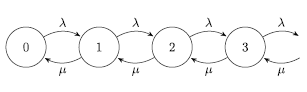
\includegraphics[width=0.5\textwidth]{Chap2_AlgorithmsPFQN/MM1_BDP.png}
\caption{Birth-death Markov process for M/M/1 queue}
\label{fig:MM1_BDP}
\end{center}
\end{figure}

\subsection{M/M/m queuing system} \label{sec:MMmQsystem}
This is a generalization of the M/M/1 system to stations with multiple servers - denoted by m. This system have service rates equal to \(\min(n,m)\mu\), where \(n\) is the instantaneous system population, and \(\mu\) is the equivalent M/M/1 service rate. The arrival process is also exponential with rate \(\lambda\). The steady state solution to the global balance equation exists if the system is stable (\(\lambda < m\mu\)), and it is given in terms of \(p_0\):
\begin{equation*}
    p_n=
    \begin{cases}
        p_0 \rho^n/n!, & n < c\\
        p_0 \rho^n/(m!m^{(n-m)}), & n \geq c
    \end{cases}
\end{equation*}
Where \(\rho = \lambda/\mu\), and the empty queue probability is given:
\[p_0 = (\sum_{n=0}^{m-1} \frac{\rho ^ n}{n!} + \frac{\rho ^ m}{(m-1)(m-\rho)})^{-1}\]

The average population of the system can be given as \(N\):
\[N = m \rho + p_m \rho / (1 - \rho)^2\]
And the mean response time \(R\):
\[R = \mu^{-1} + p_m / m \mu (1 - \rho)^2\]


\section{Queueing Networks}\label{sec:QNetworks}

Complex systems in many applications can be described in terms of a queuing network. This is a network of service centres (and variants thereof) as described above. A queuing network can be fully defined given the following inputs:
\begin{itemize}
    \item \textbf{Service centres} : The service centres have to be supplied. These service centres can be described using Kendall's notation according to the characteristics described in section \ref{sec:QueueingSystems}
    \item \textbf{Customers} : In open networks, this will be specified as an arrival distribution, whereas in closed networks, these will be described as the number of customers (these can be specified per-class in the multi-class case).
    \item \textbf{Network Topology} This describes how individual service centres connect with each other, and how customers can be routed. This is usually defined via a routing matrix. 
\end{itemize}

\subsection{Open and Closed Queuing Networks}

Open and Closed queuing networks differ in terms of how customers are available to the system. Open networks derive its customers from an external source, where arrivals are usually modelled as a Poisson arrival process. Given \(M\) service centres, this requires the specification of an external arrival rate vector \(\boldsymbol{\gamma} = (\gamma_1, \gamma_2, ... \gamma_M)\), one element per service centre. Furthermore, the routing probability matrix \(\mathbf{Q}\) \textbf{between the service centres only}, gives the traffic equations:
\[\boldsymbol{\lambda} = \boldsymbol{\gamma} + \boldsymbol{\lambda}\mathbf{Q}\]
Solving for \(\boldsymbol{\lambda}\) gives the arrival rates at individual stations in the network. \\
Closed networks, on the other hand, does not take in external arrivals, but instead circulate jobs internally. In this case, \(\boldsymbol{\gamma}\) can be set to \(\mathbf{0}\), and the traffic equations become:
\[\boldsymbol{\lambda} = \boldsymbol{\lambda}\mathbf{Q}\]
The forced-flow law also allows us to write, where \(\mathbf{v}\) is the number of visits:
\[\mathbf{v} = \mathbf{v}\mathbf{Q}\]
Since solving this entails solving a homogeneous linear system, no unique solution exists, but \(\mathbf{v}\) can usually be expressed in terms of ratios of each other, giving a set of visit ratios.

\subsection{Single-Class and Multi-Class Queuing Networks}
The analysis of queuing networks can differ depending on if a single class or multiple classes are considered. For example, in the description of service centres, the scheduling disciplines makes no difference for single class networks. However, for multi-class networks this become important. The restrictions for multi-class service centres in the context of product-form queueing networks are discussed in section \ref{sec:pfqn}. Besides, that, the concept of chains allow for jobs of different classes to switch classes within chains. However, \cite{Zahorjan1979AnNetworks} has shown that each chain can be equivalently analyzed as a single class, and multi-chain networks can be converted into an equivalent multi-class problem. Chapter 7 in \cite{Bolch2006QueueingApplications} also provides an algorithm to convert from the former to the latter network. In this project, we only consider the case where class switching is not allowed.

\subsection{Direct Solution of the Global Balance Equations}
A naive but straightforward approach to computing performance measures of queueing networks, is by modelling the network as a discrete space, continuous time homogeneous markov process. This can be done by enumerating and solving its underlying CTMC (assuming all queues are Markovian).
\\\\
Given a set of \(K\) queues, and \(R\) classes of jobs, the state space can be defined as the joint population vectors of the queues in the networks:
\begin{equation}
    \mathbf{S}_i = (\mathbf{n}_1, \mathbf{n}_2 ... \mathbf{n}_K)
\end{equation}
Where \(\mathbf{n}_k \in \mathbb{R}^R\) is the population vector of the jobs residing in service centre k.
\\\\
Let \(\mathbf{S}_{i,(nc)}\) be the population of the n-th node for class c, at state i. The transition matrix can now be defined:
\begin{equation*}
    T_{ij}=
    \begin{cases}
        \text{TR}(\mathbf{S}_i, l, c)q_{r,lk}, & \text{iff } \mathbf{S}_j \text{ is reachable from } \mathbf{S}_i \text{ through nodes l and k respectively, }\\  & \text{via the completion of a job in class c}\\
        0, & \text{otherwise}
    \end{cases}
\end{equation*}

Here \(\text{TR}(\mathbf{S}_i, l, c)\) is the (exponential) transition rate out of state \(\mathbf{S}_i\), given a class \(c\) job completes service at station l. For multi-class networks, the transition rates are, in general, station and load dependent, therefore \(\text{TR}\) is in general a function of the origin state, departing station, and departing job class. \(q_{c,lk}\) is the routing probability between nodes \(l\) and \(k\), for class c. This is covered in more detail in section \ref{sec:pfqn}.
\\\\
For a closed network with a finite number of jobs, as soon as the (finite) state space is enumerated, and the transition matrix constructed, the steady state probabilities can be computed by solving:
\begin{equation*}
    \mathbf{p}\mathbf{T'} = \mathbf{b}
\end{equation*}
Where \(\mathbf{T'}\), is the augmented transition matrix \(\mathbf{T}\) (where the last column is all 1), and \(\mathbf{b}\) is a zero vector but with the last element equals to 1, to give the normalizing condition.
\\\\
For an open network, the global balance equations will take the form of a recurrence relation similar to that of the one for the \(M/M/1\) or \(M/M/m\) queues (see sections \ref{sec:MM1Qsystem}, \ref{sec:MMmQsystem}). The solution is a closed-form expression for \(p(\mathbf{S}_i)\), the steady state probability given state \(\mathbf{S}_i\). We will focus on solution methods for closed-networks in this project.
\\\\
Given a list of states, \(\mathbf{S}_i\), the steady state probabilities \(\mathbf{p}(\mathbf{S}_i)\), performance metrics can be calculated by taking expectations and variances of various metrics such as queue lengths (\(Q_{kr}\)).
\\\\
Needless to say the solution of the (closed) network via this method is extremely costly, and grows exponentially with the number of jobs, as well as the number of service stations in the network. In the multiclass case, the size of the state space would be:
\[|\mathbf{S}| = O\bigg( \prod_c^C \binom{K_c + M -1}{K_c} \bigg)\]

Clearly this is not an option when modelling modern systems with a hundreds or thousands of service centres and classes. The idea of product form queueing networks, however, provides a convenient closed-form expression for the steady-state probability densities of a restricted, but useful class of networks, which will allow for much more efficient algorithms for performance measures.

\section{Algorithms for Product Form Queueing Networks}\label{sec:AlgorithmsPFQN}
\subsection{Product Form Queueing Networks}\label{sec:pfqn}
In this section, we introduce the notion of the product form solution for queueing networks, which will form the basis of the rest of the report. The product form solution of queueing networks expresses the steady-state probabilities of the underlying CTMC, for a single station, based on a product of the state and the parameters of individual stations. Given certain assumptions, the closed-form stationary state distribution of the CTMC is given by the product-form solution, for the single-class case as:
\begin{equation}\label{eq:pfqn_single_class}
    p(\mathbf{n}) = \frac{1}{G_{\mathbf{\theta}}} V(N) \prod_{i=1}^M g_i(n_i)
\end{equation}
Where \(\mathbf{n} = (n_1, n_2, ... n_M)\), the state of the network denoted by the number of jobs currently residing in each of the \(M\) queues. \(N = \sum_{i=1}^M n_i\). \(V(N)\) is a function of the state of the network and depend on the network's parameters and the types of service-centre/queues. \(g_i(n_i)\) is the marginal stationary queue length distribution for queue \(i\) when considered in isolation as a single queue open system. \(G = \sum_{\mathbf{n} \in \mathcal{S}_M} V(N) \prod_{i=1}^M g_i(n_i)\) is the normalizing constant of the distribution. \(\mathcal{S}_M\) is the set of all reachable states of the system. For a closed system with total population \(N\) this will be:
\[ \mathcal{S}_M = \{ \mathbf{n} \in \mathbb{N}^{MR} | n_k \geq 0, \sum_{i=1}^M n_i = N\}\]

In the special case of an open network, it can be proven that \(G=1\), and for closed networks \(V(N) = 1\). 
\\\\
For the case of a network with multiple classes of customers equation (\ref{eq:pfqn_single_class}) can be generalized to the following form:
\begin{equation}\label{eq:pfqn_multi_class}
    p(\mathbf{n}) = \frac{1}{G_{\mathbf{\theta}}} \prod_{r=1}^R V_r(N_r) \prod_{i=1}^M g_i(\mathbf{n}_i)
\end{equation}
Where \(\mathbf{n} \in \mathbb{N}^{MR}\), is the population matrix, and \(n_{kr}\) is the population of jobs of class \(r\) at station \(k\). \(V_r\) is again defined in terms of network parameters, and \(g_i\) is defined in terms of parameters of service centre \(i\) only. 

\begin{definition}
    Local balance property. A node/queue has local balance property is the departure rate from a state of of the queueing network \(\mathbf{S}_i\) due to the departure of a job of any class from node \(k\) equal to the arrival rate to this state due to an arrival of another job to the same node.
\end{definition}

The local balance property implies that the global balance equations for a state can be partitioned into a set of separate balance equations. A solution to the local balance equations is therefore also a solution to the global balance equations (the converse is not always true). \cite{Chandy1977ProductNetworks} proved that if a network only has nodes satisfying the local balance property, the network has a product form solution for the stationary state distribution.
\\\\
Two important results derived a product form solution for the case of a single-class open network (Jackson's theorem \cite{Jackson2004Jobshop-LikeSystems}), and a single-class closed network (the Gordon-Newell theorem \cite{Gordon1967ClosedServers}). 
\\\\
To introduce Jackson's theorem, we first consider a Jackson network. These are open networks of queueing systems which satisfy the following conditions:
\begin{itemize}
    \item The network has infinite capacity
    \item Every node in the network is \(M/M/m_i-FCFS\), where node \(i\) has \(m_i\) identical servers
    \item Every node in the network can have Poisson arrivals from outside, and a customer can leave the system from any node.
\end{itemize}
\begin{theorem}
    Jackson's theorem states that, a stable Jackson network consisting only of \(M/M/1-FCFS\) queues, (i.e. \(\lambda_i < \mu_i \; \forall i = 1, .. M\)), the product form solution of the network is given:
    \begin{equation}
        P(\mathbf{n}) = \prod_{i=1}^M (1-\rho_i) \rho_i^{n_i}
    \end{equation}
\end{theorem}

The Gordon-Newell theorem extends this result to a closed-system of \(M/M/m-FCFS\) queues with a fixed number of customers \(N\).
\begin{theorem}
    The Gordon-Newell theorem for closed-networks of single-class \(M/M/m-FCFS\) queues states that the stationary state probability this network is given by the product form solution:
    
    \begin{equation}\label{eq:GNPFQN}
        P(\mathbf{n}) = \frac{1}{G_{\boldsymbol{\theta}}(N)} \prod_{i=1}^M \bigg( \frac{\theta_i^{n_i}}{\prod_{j=1}^{n_i} \beta_i(j)} \bigg)
    \end{equation}
    
    Where \(\theta_i\) is the service demand placed on node \(i\) by a single job, given by the utilization law, where \(\lambda(N)\) is the overall throughput of the system:
    \begin{equation*}
        \theta_i = \rho_i \lambda(N)
    \end{equation*}
    
    And \(\beta_i(j) = \min(m_i, j)\) is a scaling factor for nodes with \(m_i\) servers.
    
    The normalizing constant \(G_{\boldsymbol{\theta}}(N)\) is given by summing the product terms in equation (\ref{eq:GNPFQN}).
    
\end{theorem}

\begin{proof}
    The proof of the above theorems involve showing that the formulas for \(P(\mathbf{n})\) above satisfy the global balance equations for the underlying CTMC. This is given in full in \cite{Bolch2006QueueingApplications} Chapter 7.
\end{proof}

The BCMP theorem, named after the authors that first theorized it \cite{Baskett1975OpenCustomers}, , expanded the product form solution even further to include multi-class networks and networks of types other than \(M/M/m-FCFS\) servers. These are grouped into 4 types of networks, collectively referred to as BCMP networks.

\begin{definition}
    BCMP networks are open, closed or mixed multiclass networks that consist of queues which fall into one of the following types:
    \begin{itemize}
        \item \textbf{Type 1:} FCFS queuing discipline \(-/M/m-FCFS\). For multiclass networks, all job classes must have the same service rate \(\mu_i\).
        \item \textbf{Type 2:} Processor-sharing (PS) queuing discipline and arbitrary phase-type distribution \(-/G/1-PS\)
        \item \textbf{Type 3:} Infinite server (IS) and arbitrary phase-type distribution -/G/\(\infty\)
        \item \textbf{Type 4:} Last come first serve with pre-emptive resume (LCFS-PR) and arbutrary phase-type distribution \(-/G/1-LCFS\).
    \end{itemize}
\end{definition}

\begin{theorem}
    The BCMP theorem states that, for BCMP networks, the steady state product form solution is given by :
    \begin{equation} \label{eq:BCMP_PFQN}
        p(\mathbf{n}) = \frac{1}{G_{\boldsymbol{\theta}}(\mathbf{N})} \prod _ {i=1} ^ M F_i(\mathbf{n_i})
    \end{equation}
    Where \(\mathbf{n} = (\mathbf{n}_1, ... \mathbf{n}_M)\) And the function \(F_i(\mathbf{n}_i)\) is given by:
    \begin{equation}
        F_i(\mathbf{n}_i)=
        \begin{cases}
            \frac{1}{\beta_i(n_i)} n_i! \prod _{r=1} ^ R  \frac{\theta_{ir}^{k_{ir}}}{n_{ir}!} & \text{Type 1}\\\\
            k_i! \prod _{r=1} ^ R  \frac{\theta_{ir}}{(k_{ir}!)} & \text{Type 2,4}\\\\
            \prod _{r=1} ^ R \frac{\theta_{ir}}{(k_{ir}!)} & \text{Type 3}\\
        \end{cases}
    \end{equation}
    Where the job service demands \(\theta_{ir}\) can be expressed in terms of visit ratios and service rates:
    \begin{equation*}
        \theta_{ir} = \frac{v_{ir}}{\mu_{ir}}
    \end{equation*}
\end{theorem}

The proof of this theorem is complex and outside of the scope of this project. The original proof \cite{Baskett1975OpenCustomers} was given by the authors of the theorem and involved checking that the local and global balance equations of the underlying CTMC are satisfied by the above product form solution.

\subsection{The Normalizing Constant and Performance Indices}
The normalizing constant \(G\) of the product-form solution for queueing networks is of paramount importance in applications involving network modelling. Not only does this quantity allow us to compute the actual steady-state probabilities of the network, it arises in the computation of network performance indices such as the average queue length \(Q_{kr}\), and overall class throughputs \(\lambda_r\). For closed queueing networks, this is given \cite{Reiser1975QueuingAlgorithms}:

\begin{equation}
    \lambda_r(\mathbf{N}) = \frac{G_{\boldsymbol{\theta}}(\mathbf{N} - \mathbf{1}_r)}{G_{\boldsymbol{\theta}}(\mathbf{N})}
\end{equation}
\begin{equation}
    Q_{kr}(\mathbf{N}) = \theta_{kr} \frac{G^{(+k)}_{\boldsymbol{\theta}}(\mathbf{N} - \mathbf{1}_r)}{G_{\boldsymbol{\theta}}(\mathbf{N})}
\end{equation}

Where \(\mathbf{1}_r \in \mathbb{N}^r\) is a vector that has all zeros except for a \(1\) in position \(r\). \(G^{(+k)}_{\boldsymbol{\theta}}(\mathbf{N})\) Is the normalizing constant for a network augmented with an extra node \(k\). Average response times and utilizations can be computed in terms of \(Q_{kr}(\mathbf{N})\) and \(\lambda_r(\mathbf{N})\) via the application of the fundemental laws, e.g. Little's Law and the Utilization Law.
\\\\
While it is true that there are algorithms \cite{Reiser1975QueuingAlgorithms, Chow1983ApproximationsNetworks, Chandy1982Linearizer:Systems, Sevcik2002SolutionAlgorithm} that can compute these average performance indices, \(Q_{kr}\) and \(\lambda_r\), more efficiently than \(G\) can be computed, there are still many explicit uses of \(G\) of interest. 
\\\\
Casale \cite{Casale2017AcceleratingMethods} provides one such motivating example. Suppose we are provided with a set of \(L\) state samples \(\mathbf{n}^{(l)} \in \mathcal{S}_M, \; l=1,...L\), assuming zero delays, and a network of single-server nodes, the log-likelihood of the samples given a demand matrix \(\boldsymbol{\theta}\) ( (\(\log P(\{\mathbf{n}^{(l)} \forall l=1,...L \} | \boldsymbol{\theta})\) or \(\mathcal{L}(\boldsymbol{\theta})\) ) can be written:
\[\mathcal{L}(\boldsymbol{\theta}) = \sum_{l=1}^L \log C(\mathbf{n}^{(l)}) + L \sum_{k} \sum_{r} \widetilde{Q}_{kr} \log \theta_{kr} - L \log G_{\boldsymbol{\theta}}(\mathbf{N})\]

Where \(\widetilde{Q}_{kr} = \sum_{l} n_{kr}^{(l)}/L\) is the \textit{measured} mean queue-length of class \(r\) at node \(k\).

\subsection{Exact Algorithms}\label{sec:exact_algos}
\textit{{\large Convolution Algorithm}}\\\\
The Convolution Algorithm (CA) makes use of the product form solution of the networks described in \ref{sec:pfqn} to compute the normalizing constant \(G_{\boldsymbol{\theta}}(\mathbf{N})\). Given a product-form solution of a closed product-form queueing network:
\begin{equation}
    p(\mathbf{n}) = \frac{1}{G_{\boldsymbol{\theta}}(\mathbf{N})} \prod_{k=1}^M g_i(\mathbf{n}_i)
\end{equation}

Where the normalizing constant \(G_{\boldsymbol{\theta}}(\mathbf{N})\) can be given in the explicit summation, (Where \(N_r\) is the total population of jobs of class \(r\)):
\[G_{\boldsymbol{\theta}}(\mathbf{N}) = \sum_{\substack{\mathbf{n} \geq \mathbf{0}\\ \sum_r{n_{kr}} = N_r}} \prod_{i=1}^M g_i(\mathbf{n_i})\]

This can be re-arranged to give the following recursive summation:
\[ G_{\boldsymbol{\theta}}(M, \mathbf{N}) =  \sum_{\mathbf{0} \leq \mathbf{j} \leq \mathbf{N}} g_i(\mathbf{j}) G_{\boldsymbol{\theta}}(M-1, \mathbf{N-j})\]

Where \(G_{\boldsymbol{\theta}}(M-1, \mathbf{N})\) is the normalizing constant for a network with the \(M^{th}\) queue removed. And the initial conditions are as follows:
\[G_{\theta}(1,\mathbf{N}) = g_1(\mathbf{n}_1) \quad G_{\theta}(\cdot,\mathbf{0}) = 1\]
For a model consisting only of load independent stations, the equation simplifies to:
\[G_{\boldsymbol{\theta}}(M, \mathbf{N}) = G_{\boldsymbol{\theta}}(M-1, \mathbf{N}) + \sum_{r=1}^R \theta_{kr} G_{\boldsymbol{\theta}}(M, \mathbf{N-1_r}) \]

This method, while far more efficient than the explicit summation of the terms for each state, still grows like \(O(\prod_{r=1}^R N_r^2)\) for the general case, and \(O(MR \prod_{r=1}^R N_r)\) in the case with load-independent demands. Space requirements = \(O(\prod_{r=1}^R N_r)\), like the number of subproblems.
\\\\
\textit{{\large Mean Value Analysis Algorithm}}\\\\
The mean value analysis (MVA) algorithm first presented in \cite{Reiser1980Mean-ValueNetworks} bypasses the need to compute the normalizing constant, and instead computes the average performance indices directly, through a multi-dimensional recursion. The MVA algorithm is given here for BCMP networks.
\\\\
This is defined as follows \cite{Lazowska1984QuantitativeModels}:
The node residence time \(W_{kr}(\mathbf{N})\) is given:
\begin{equation}\label{eq:MVA_step1}
    W_{kr}(\mathbf{N}) = 
    \begin{cases}
        \theta_{kr} & \text{if node k is a Type 3 node}\\
        \theta_{kr}(1 + A_{kr}(\mathbf{N})) & \text{if node k is a Type 1,2 or 4 node, } m_k = 1\\
        \frac{\theta_{kr}}{m_i}(1 + A_{kr}(\mathbf{N})) & \text{if node k is a Type 1 node, } m_k > 1
    \end{cases}
\end{equation}
Where \(A_{kr}(\mathbf{N})\) is the arrival instant queue length for class \(r\) at node \(k\). Turns out there are several techniques to obtain an exact and approximate solution to this set of equations, and that lies in the way \(A_{kr}(\mathbf{N})\) is computed.
\\\\
The other equations involved in this recursion is based on Little's Law:
\begin{equation}\label{eq:MVA_step2}
  \lambda_{r}(\mathbf{N}) = \frac{N_r}{\sum_{k=1}^M} W_{kr}(\mathbf{N})  
\end{equation}
\begin{equation}\label{eq:MVA_step3}
K_{kr}(\mathbf{N}) = \lambda_{r}(\mathbf{N}) W_{kr}(\mathbf{N})
\end{equation}

In exact MVA, \(A_{kr}(\mathbf{N})\) is calculated exactly according to the following equation:
\[A_{kr}(\mathbf{N}) = 
\begin{cases} 
Q_{kr}(\mathbf{N-1_r}) & \text{Type 1,2,4 nodes, with }m_k = 1 \\ 
Q_{kr}(\mathbf{N-1_r}) + \sum_{j=0}^{m_i-2} (m_k - j - 1)p_k(j|\mathbf{N-1_r}) & \text{Type 1 nodes, with } m_k = 1
\end{cases}
\]
Here the marginal probability that there are \(j\) jobs at the \(k^{th}\) node, \(0 \leq j \leq m_i-1\) given that the network is in state \(\mathbf{N>0}\)
\[
p_k(j|\mathbf{N}) = 
\begin{cases} 
\frac{1}{j} \bigg[ \sum_{k=1}^R \theta_{kr} \lambda_r(\mathbf{N}) p_k(j-1|\mathbf{N-1_r}) \bigg] & j > 0\\ 
1 - \frac{1}{m_k} \bigg[ \sum_{r=1}^R \theta_{kr} \lambda_r(\mathbf{N}) + \sum_{j=1}^{m_k-1}(m_k - j)p_k(j|\mathbf{N})\bigg]  & j=0 
\end{cases}
\]
And base case:
\[ p_k(j|\mathbf{0}) =  \begin{cases} 1  & j=0 \\ 0 & \text{otherwise} \end{cases} \]
The time complexity of this algorithm is \(O(RM \prod_{r=1}^R N_r)\), and the space complexity is \(O(M \prod_{r=1}^R N_r)\). Both time and space complexity for MVA is also exponential in the number of classes, but grows less quickly for the load-dependent (multiserver/IS) case than the convolution algorithm.
\\\\
The approximate solution of \(A_{kr}(\mathbf{N})\) will be discussed in section \ref{sec:approx_algos}. 
\\\\
\textit{{\large RECAL Algorithm}}
\\\\
In this algorithm, first presented in \cite{Conway1986RECAL---aNetworks}, each queue is completely associated with a single, self-looping class. The RECAL algorithm uses the following recursion algorithm:
\begin{equation}
    N_r G_{\boldsymbol{\theta}}(\mathbf{m,N}) = \sigma_r G_{\boldsymbol{\theta}}(\mathbf{m,N-1_r}) + \sum_{k=1}^M (1 + m_k) \theta_{kr} G_{\boldsymbol{\theta}}(\mathbf{m+1_k,N-1_r})
\end{equation}
Where \(G_{\boldsymbol{\theta}}(\mathbf{m,N})\) is the normalizing constant of a queueing network of load-independent servers, and \(\mathbf{m} \in \mathbb{N}^M\) is the multiplicity vector indicating the count of the number of each server. \(\sigma_r\) indicates the mean delay experienced by each class in the network. The initial conditions are given:
\[G(\mathbf{0}, \mathbf{N}) = \prod_{r=1}^R \frac{\theta_r^{N_r}}{N_r!} \quad G(\cdot, \mathbf{0}) = 1 \]
\\\\
This algorithm has time and space complexity \(O(N^M)\), making it suitable only for networks with a small number of queues.
\\\\
\textit{{\large Method of Moments Algorithm}}\\\\
A number of variants of this method exists, given in \cite{Casale2011ANetworks, Casale2011ANetworksb, Casale2009CoMoM:Models}. This method applies the convolution algorithm and RECAL algorithm to a set of normalizing constants that differ for the lements and compotision of \(\boldsymbol{\theta}\) and \(\mathbf{N}\). Different rules exist to define this set of normalizing constants, called the \textit{basis}. Given that the normalizing constants in the basis are given in the vector \(\mathbf{g(N)}\), the method of moments defines a matrix recurrence relation.
\[\mathbf{A(\boldsymbol{\theta}, N)g(N)} = \mathbf{B(\boldsymbol{\theta}, N)g(N-1_r)}\]
For any \(1 \leq r \leq R\), and \(\mathbf{g(0)}\) are given by the initial conditions as defined in the convolution and RECAL algorithms. The square matrices \(\mathbf{A(\boldsymbol{\theta}, N)g(N)}\) and \(\mathbf{B(\boldsymbol{\theta}, N)g(N)}\) are square matrices, and decrease in size as the recurrence progresses. 
\\\\
Provided that \(\mathbf{A(\boldsymbol{\theta}, N)}\) is invertible at all steps of the recursion, it is possible to compute \(\mathbf{g(N)}\) and obtain \(\mathbf{G_{\boldsymbol{\theta}}(N)}\) from the elements of \(\mathbf{g(N)}\). A required condition for invertibility if that \(\theta_{ir} \neq \theta_{jr}, \forall i,j,r, i \neq j\). This algorithm has a theoretical time complexity of \(O(N)\) time and \(O(1)\) space. However, since the method of moments algorithm requires the above recurrence relation to be carried out using exact arithmetic, a significant portion of the cost could go to performing calculations using exact representations.

\subsection{Approximate and Randomized Algorithms} \label{sec:approx_algos}

\textit{{\large Approximate Mean Value Analysis Algorithm}}\\\\
Approximate Mean Value Analysis (AMVA) algorithms work by providing a reasonable estimate to the arrival instant queue lengths \(A_{kr}(N)\). In exact MVA, this was computed using exact recursion. The Chow algorithm \cite{Chow1983ApproximationsNetworks} approximates this as:
\[A_{kr}(\mathbf{N}) = Q_{kr}(\mathbf{N-1_r}) \approx Q_{kr}(\mathbf{N}) \]
Based on the assumption that the average queue lengths for a network with one less customer is almost identical to that of a network with one less customer. This assumption is reasonable for a model with a large number of customers.
\\\\
The above approximation can be then used in the system of equations (\ref{eq:MVA_step1}, \ref{eq:MVA_step2}, \ref{eq:MVA_step3}), which can be solved iteratively until the required tolerance between values of successive iterations falls below a certain threshold.
\\\\
The Brad-Schweitzer Algorithm \cite{Schweitzer1993AQueues} provides a slightly better approximation to \(A_{kr}(\mathbf{N})\):
\[Q_{kr}(\mathbf{N-1_r}) = \frac{N_r-1}{N_r} Q_{kr}(\mathbf{N}) + \sum_{\substack{j=1\\ j\neq r}}^R Q_{kr}(\mathbf{N})\]
Which provides more accurate esimates than the Chow AMVA algorithm at the cost of additional computation complexity per iteration. Better approximations to the MVA system of equations are provided in \cite{Chandy1982Linearizer:Systems} which include performing calculations of \(O(MR^2)\) to obtain even better approximations at the cost of more complexity.
\\\\
\textit{{\large Monte Carlo Methods}}\\\\ 
Monte Carlo integration methods for the normalizing constant were first introduced in \cite{Ross1994MonteNetworks}. These randomized methods use the following integral form derived in \cite{McKenna1984AsymptoticNetworks}. 
\begin{equation}\label{eq:MCI_form_Ross}
    G_{\boldsymbol{\theta}}(\mathbf{N}) = \frac{1}{\prod_{i=1}^R N_r!} \int_{\mathbb{R}_+^K} e^{-y} \prod_{r=1}^R \bigg( \sigma_r + \sum_{k=1}^K \theta_{kr} y_k \bigg)^{N_r} d \mathbf{y}
\end{equation}

Where \(\mathbb{R}_+^K = \{ \mathbf{y} \in \mathbb{R}^K | \mathbf{y \geq 0}\} \) is the non-negative orthant of the K-dimensional real space, \(\mathbb{R}^K\), and \(y = \sum_k y_k\). \(\sigma_r = \sum_{k=K+1}^M \theta_{kr}\) is the sum of the class-\(r\) demands at all infinite servers. The above expression is obtained by considering the form of the normalizing constant for networks of single and infinite server queues only:
\begin{equation*}
    G_{\boldsymbol{\theta}}(\mathbf{N}) = \sum_{\mathbf{n} \in \mathcal{S}_M} \prod_{i=1}^K n_i! \prod_{k=1}^M \prod_{r=1}^R \frac{\theta_{n_{kr}}}{n_{kr}!}
\end{equation*}

Expression (\ref{eq:MCI_form_Ross}) is obtained by expression the \(n_i!\) terms in the above form of the normalizing constant, in the integral form of the gamma function, and subsequently by repeated application of the multinomial theorem:
\begin{equation*}
    \bigg( \sum_{k=1}^K x_k \bigg)^V = V! \sum_{\mathbf{v \geq 0}, v=V} \prod_{k=1}^K \frac{x_k}{v_k!}
\end{equation*}

The integral form of the normalizing constant (\ref{eq:MCI_form_Ross}) can be efficiently evaluated using importance sampling with the following sampling distribution:
\[p(\mathbf{y}) = \prod_{i=k}^K p_k(y_k)\]
And \(p_k(y_k)\) is the PDF of a scalar exponential distribution:
\[p_k(y) = \gamma_k e^{-\gamma_k y}\]
Where \(\gamma_k\) are parameters that can be tuned to minimize variance in the computed integral \cite{Ross1994MonteNetworks}. Typically a sample size of \(10^5-10^7\) is required in order to approximate \(G_{\boldsymbol{\theta}}(\mathbf{N})\) with reasonable variance. 
\\\\
In a similar vein to \cite{Ross1994MonteNetworks}, this project focuses on applying Monte Carlo integration of an integral form of the normalizing constant. However, unlike what has been done before, this project builds on novel integral forms of the normalizing constant \(G_{\boldsymbol{\theta}}(\mathbf{N})\) to achieve a better sampling efficiency than what was achieved in previous randomized methods. These will be described in detail in the following chapters.



%%%%%%%%%%%%%%%%%%%%%%%%%%%%%%%%%%%%
\chapter{Integrals On the Simplex}\label{sec:Chapter3}

In this chapter, novel integral forms of the normalizing constant for 3 types of networks are presented: single-server networks (section \ref{sec:single_server_simplex_integral}), single-server networks with delay(section \ref{sec:inf_server_simplex_integral}), and multi-server networks (section \ref{sec: multi_server_simplex_integral}), with the main results being presented in equations (\ref{eq:start_simplex_single_server}), (\ref{eq:start_simplex_inf_server}), and (\ref{eq:multi_server_NC}), respectively. These take the form of integrals of functions over the \(K\)-dimensional unit simplex (denoted by \(\Delta_K\) or \(\mathbb{S}^K\)), for a network with \(K\) nodes/queues.
\\\\
These integral forms of the normalizing constant \(\mathbf{G}_{\boldsymbol{\theta}}(\mathbf{N})\) forms the basis of this project's approach, and will be used and referenced extensively throughout this report.
\\\\
The original proofs of the single-server and single and infinite (delay) server networks were given in \cite{Casale2017AcceleratingMethods}. Here, an alternative proof is presented, which uses the Dirichlet Integral identity over the simplex in equation (\ref{eq:dirichlet_simplex_integral}). 

\section{Preliminaries}

The purpose of this section is to summarize several important identities that are required to derive the simplex integral form of the normalizing constant.
\\\\
The multinomial theorem states that, for any set of real numbers \((x_1, x_2 ... x_k)\), and nonnegative integer \(V\):
\begin{equation}\label{eq:mt}
    \bigg( \sum_{k=1}^K x_k \bigg)^V = V! \sum_{\substack{\mathbf{v} \geq 0, \\ \sum_k^K v_k = V}}\prod_{k=1}^K \frac{x_k^{v_k}}{v_k!}
\end{equation}

\begin{theorem} \label{theorem:multinomial_2}
The multinomial theorem implies the following. For any set of real numbers \((a_1, a_2 ... a_k)\), and nonnegative integer \(N\)
    \begin{equation} \label{eq:multinomial_2}
        a_1^{N_1} a_2^{N_2} ... a_R^{N_R} = \frac{1}{N!} \frac{\partial^{N_1}....\partial^{N_R}}{\partial t_1^{N_1}....\partial t_R^{N_R}}\bigg( \sum_{i=1}^R a_i t_i \bigg)^N
    \end{equation}
\end{theorem}

\begin{proof}
    Taking the term on the right hand side of (\ref{eq:multinomial_2}), using (\ref{eq:mt}), we can write:
    \begin{equation}\label{eq:differentiation_filter}
        \frac{1}{N!} \frac{\partial^{N_1}....\partial^{N_R}}{\partial t_1^{N_1}....\partial t_R^{N_R}}\bigg( \sum_{i=1}^R a_i t_i \bigg)^N = \frac{1}{N!} \frac{\partial^{N_1}....\partial^{N_R}}{\partial t_1^{N_1}....\partial t_R^{N_R}} \bigg( N! \sum_{\substack{\mathbf{n} \geq 0, \\ \sum_i^R n_r = N}}\prod_{i
        =1}^R \frac{(a_i t_i)^{n_i}}{n_i!} \bigg)
    \end{equation}
    And the fact that 
    \begin{equation*}
        \frac{\partial^{N_i}}{\partial t_i ^{N_i}} \prod_{i=1}^R t^{n_i} = 
        \begin{cases}
             \prod_i^R N_i! & \text{if } n_i = N_i, \forall i=1...R \\
            0 & \text{otherwise}
        \end{cases}
    \end{equation*}
    
    We recover the left hand side of (\ref{eq:multinomial_2}).
    
\end{proof}

Another important result is the identity of the definite integral over the simplex \(\Delta_K\):
\begin{equation} \label{eq:dirichlet_simplex_integral}
    \int_{\Delta_K} \prod_{k=1}^K u_k^{n_k} d\mathbf{u} = \frac{\prod_{k=1}^K n_k!}{\big( \sum_{k=1}^K n_k +K -1 \big)!}
\end{equation}
 The \(K\)-dimensional unit simplex is defined as a set of \(K\)-dimensional points \(\mathbf{u}\) in the positive quadrant, such that all such points have sum of their components equal to 1:
 \begin{equation*}
    \Delta_K = \bigg  \{ \mathbf{u} : \forall u_i > 0, \sum_{i=1}^K u_i = 1 \bigg \}
\end{equation*}
\subsection{Finite Differences}

Another important concept required for the derivation of results in section \ref{sec: multi_server_simplex_integral} is that of finite differences. It may be seen as the discrete analog of continuous derivatives in calculus. 

\begin{definition}
    For a discrete function \(f_k\), defined at discrete points \(k \geq 1\) The \(n\)-th forward difference of a function is given by the recurrence relation:
    \[\Delta_k^n = \Delta_k^{n-1} f_{k+1} - \Delta_k^{n-1} f_{k}\]
    Where the first-order difference is given:
    \[\Delta_k f_k = f_{k+1} - f_k\]
\end{definition}

An alternative formulation of the forward difference is that of the alternating sum:
\begin{equation}
    \Delta_k^n f_k = \sum_{k=0}^n (-1)^{n-k} \begin{pmatrix} n \\ k\end{pmatrix} f_k
\end{equation}

A result of Euler's formula for \(n\)-th differences of powers is given in \cite{Gould1978EulersPowers} for the case where \(f_k\) is a polynomial of the form \(k^m\):
\begin{equation}\label{eq:euler_power_diffrences}
    \Delta_k^n k^m = \sum_{k=0}^n (-1)^{n-k} \begin{pmatrix} n \\ k\end{pmatrix} k^m = 
    \begin{cases}
    0 & \text{if } m < n \\
    n! & \text{if } m=n
    \end{cases}
\end{equation}

To generalize to multivariate polynomials \(p(\mathbf{k})\), where \(\mathbf{k} = (k_1, ... k_m)\), we introduce the notation for the composition of \(m\) forward differences:
\begin{equation}
    \Delta_\mathbf{k}^\mathbf{n} p(\mathbf{k}) = \Delta_{k_m}^{n_m} \Delta_{k_{m-1}}^{n_{m-1}} ... \Delta_{k_1}^{n_1} p(\mathbf{k})
\end{equation}

The repeated application of Euler's formula (\ref{eq:euler_power_diffrences}) on each \(\Delta^n_k\) operator leads to the following proposition from \cite{Casale2018ExplicitRepresentations}:
\begin{theorem} \label{theorem:multivar_euler_power_differnces}
    Let \(p(\mathbf{k})\) be a polynomial of degree \(n = n_1 + ... + n_m\) in the discrete variable \(\mathbf{k} = (k_1, ... k_m)\). If we denote the coefficient of the monomial \(k_1^{n_1}k_2^{n_2}...k_M^{n_m}\) as \(a_0\) , then
    \begin{equation}
        \Delta_\mathbf{k}^\mathbf{n} p(\mathbf{k}) = \sum_{\mathbf{0 \geq k \neq n}} (-1)^{n-k} \prod_{i=1}^m \begin{pmatrix} n_i \\ k_i \end{pmatrix} p(\mathbf{k}) = a_0 \prod_{i=1}^m n_i!
    \end{equation}
\end{theorem}

A formal, inductive prove on the above theorem is given in \cite{Casale2018ExplicitRepresentations}. A consequence of the above theorem is that for set of \(m\) arbitrary coefficients \(\mathbf{u} = (u_1, ... , u_m)\):
\begin{equation}\label{eq:power_differences_multinomial}
    \frac{1}{n!} \Delta_{\mathbf{k}}^{\mathbf{n}} \bigg( \sum_{i=1}^m k_i u_i\bigg)^n =
    \frac{1}{n!} \Delta_{\mathbf{k}}^{\mathbf{n}} \sum_{\substack{\mathbf{v \leq 0} \\ v=n}} \frac{n!}{\prod_{j=1}^m v_j!} \prod_{i=1}^m k_i^{v_i} u_i^{v_i} = \prod_{i=1}^m u_i^{n_i}
\end{equation}

\section{Integral form for Single Server Node Networks} \label{sec:single_server_simplex_integral}

The integral form for single-server node networks over the \(K\)-dimensional unit simplex \(\Delta_K\) is given in the theorem below, and a proof is presented:

\begin{theorem} \label{theorem:simplex_single_server}
In a multiclass closed queueing network with K single-server nodes
    \begin{empheq}[box=\mymath]{equation}\label{eq:start_simplex_single_server}
        G_{\boldsymbol{\theta}}(\mathbf{N}) =  \frac{(N+K-1)!}{N_1! ... N_R!} \int_{\Delta_K}\prod_{r=1}^R \bigg( \sum_{k=1}^K \theta_{kr} u_k \bigg)^{N_r} d\mathbf{u}
    \end{empheq}
Where \(\Delta_K = \{ \mathbf{u} \in \mathbb{R}^K | u_i \geq 0, \sum_{i=1}^K u_i = 1\}\) is the unit simplex.
\end{theorem}

\begin{proof}
    We prove that (\ref{eq:start_simplex_single_server}) is equivalent to the original form of the normalizing constant:
    \begin{equation}\label{eq:end_proof}
    G_{\boldsymbol{\theta}}(\mathbf{N}) =  \sum_{\substack{n_{kr} \geq 0 \\ \sum_k n_{kr} = N_r \\ \forall r= 1...R}} \prod_{i=1}^{K} n_i! \prod_{k=1}^{M} \prod_{r=1}^{R} \frac{\theta_{kr}^{n_{kr}}}{n_{kr}!}
    \end{equation}
    
    Where \(\mathbf{N} = (N_1, N_2 \dot ,N_R)\). And \(N = \sum_r^R N_r\). 
    \\\\
    Starting from (\ref{eq:start_simplex_single_server}), we first write the integral on the right hand side as:
    \begin{equation*}
        I_{\boldsymbol{\theta}}(\mathbf{N}) =  \int_{\Delta_K}\prod_{r=1}^R \bigg( \sum_{k=1}^K \theta_{kr} u_k \bigg)^{N_r} d\mathbf{u}
    \end{equation*}
    
    Using the multinomial theorem of the form (\ref{eq:multinomial_2}), this can be written (after exchanging the order of integration and differentiation)
    \begin{equation}
        I_{\boldsymbol{\theta}}(\mathbf{N}) =  \frac{1}{N!} \frac{\partial^{N_1}....\partial^{N_R}}{\partial t_1^{N_1}....\partial t_R^{N_R}} \int_{\Delta_K}  \bigg( \sum_{r=1}^R \sum_{k=1}^K \theta_{kr} u_k t_r \bigg)^{N} d\mathbf{u}
    \end{equation}

    Applying the multinomial theorem (\ref{eq:mt}) on the sum in the brackets, we get:
    \begin{equation}
        I_{\boldsymbol{\theta}}(\mathbf{N}) =  \frac{1}{N!} \frac{\partial^{N_1}....\partial^{N_R}}{\partial t_1^{N_1}....\partial t_R^{N_R}} \int_{\Delta_K} N! \sum_{n_{kr} \geq 0 \\ \sum n_{kr} = N} \prod_{r=1}^R \prod_{k=1}^K \frac{\big(  \theta_{kr} u_k t_r \big)^{n_{kr}}}{n_{kr}!} d\mathbf{u}
    \end{equation}
    
    The integrand then becomes (after switching integration and summation, and factorising out \(u_k\)):
    \begin{equation}
        I_{\boldsymbol{\theta}}(\mathbf{N}) = \frac{\partial^{N_1}....\partial^{N_R}}{\partial t_1^{N_1}....\partial t_R^{N_R}}  \sum_{n_{kr} \geq 0 \\ \sum n_{kr} = N} \int_{\Delta_K} \prod_{k=1}^K u_k^{n_k} d\mathbf{u} \prod_{r=1}^R \prod_{k=1}^K \frac{\big(  \theta_{kr} t_r \big)^{n_{kr}}}{n_{kr}!} 
    \end{equation}
    
    Using (\ref{eq:dirichlet_simplex_integral}) this becomes:
    \begin{align}
        %%%%%%
        I_{\boldsymbol{\theta}}(\mathbf{N}) 
        & = \frac{\partial^{N_1}....\partial^{N_R}}{\partial t_1^{N_1}....\partial t_R^{N_R}}  \frac{1}{(N+K-1)!}  \sum_{\substack{n_{kr} \geq 0 \\ \sum n_{kr} = N}} \prod_{k=1}^K n_k! \prod_{r=1}^R \prod_{k=1}^K \frac{\big(  \theta_{kr} t_r \big)^{n_{kr}}}{n_{kr}!} \\
        %%%%%%
        & = \frac{\partial^{N_1}....\partial^{N_R}}{\partial t_1^{N_1}....\partial t_R^{N_R}}  \frac{1}{(N+K-1)!}  \sum_{\substack{n_{kr} \geq 0 \\ \sum n_{kr} = N}} \prod_{r=1}^R t_r^{n_r} \prod_{k=1}^K n_k! \prod_{r=1}^R \prod_{k=1}^K \frac{ \theta_{kr}^{n_{kr}}}{n_{kr}!} 
    \end{align}
    
    Using \ref{eq:differentiation_filter}, the terms in the summation where \(n_r \neq N_r, \forall r=1...R\) goes to zero, and we are left with
    \begin{equation}
        I_{\boldsymbol{\theta}}(\mathbf{N}) 
        = \frac{N_1!N_2!...N_R!}{(N+K-1)!}  \sum_{\substack{n_{kr} \geq 0 \\ \sum_k n_{kr} = N_r \\ \forall r= 1...R}} \prod_{k=1}^K n_k! \prod_{r=1}^R \prod_{k=1}^K \frac{ \theta_{kr}^{n_{kr}}}{n_{kr}!} 
    \end{equation}
    
    Combining this back with :
    \begin{equation}
        G_{\boldsymbol{\theta}}(\mathbf{N}) =  \frac{(N+K-1)!}{N_1! ... N_R!} I_{\boldsymbol{\theta}}(\mathbf{N}) 
    \end{equation}

    Gives us the original form of the normalizing constant (\ref{eq:end_proof}). 
\end{proof}

\section{Integral form for Networks with Infinite Server Nodes} \label{sec:inf_server_simplex_integral}

In this section, we prove the integral form for single-server node networks with infinite (delay) server present.

\begin{theorem}
In a multiclass closed queueing network with M nodes in total : K single-server nodes, and \(M-K\) infinte server nodes. The normalizing constant can be expressed by the integral:
    \begin{empheq}[box=\mymath]{equation}\label{eq:start_simplex_inf_server}
        G_{\boldsymbol{\theta}}(\mathbf{N}) =  \int_{\Delta_K} \int_{v=0}^{\infty} \frac{e^{-v} v^{K-1}}{N_1! ... N_R!} \prod_{r=1}^R \bigg( \sigma_r + v \sum_{k=1}^K \theta_{kr} u_k \bigg)^{N_r} dv d\mathbf{u} 
    \end{empheq}
    Where \(\sigma_r = \sum_{k=K+1}^M \theta_{kr}\), the sum of the infinite server node demands per class.
\end{theorem}

\begin{proof}
    We can write (\ref{eq:start_simplex_inf_server}) as:
    \begin{equation}
        G_{\boldsymbol{\theta}}(\mathbf{N}) = \frac{1}{N_1! ... N_R!} \mathbf{I(N)}
    \end{equation}
    Where:
    \begin{equation}
        \mathbf{I(N)} = \int_{\Delta_K} \int_{v=0}^{\infty} e^{-v} v^{K-1} \prod_{r=1}^R \bigg( \sum_{k=1}^M \theta_{kr} q_k \bigg)^{N_r} dv d\mathbf{u} 
    \end{equation}
    \[q_k = 
    \begin{cases}
        u_k v & k \leq K\\
        1 & k > K\\
    \end{cases}\]
    
    Using the multinomial theorem (\ref{eq:mt}) and (\ref{eq:multinomial_2}) in the same way as it was used in section \ref{sec:single_server_simplex_integral}, we can write:
    \begin{equation}
        \mathbf{I(N)} = \frac{\partial^{N_1}....\partial^{N_R}}{\partial t_1^{N_1}....\partial t_R^{N_R}} \sum_{\substack{n_{kr} \geq 0 \\ \sum n_{kr} = N}} \int_{\Delta_K} \int_{v=0}^{\infty} e^{-v} v^{K-1} \prod_{r=1}^R \prod_{k=1}^M \frac{(\theta_{kr} t_r q_k)^{n_{kr}}}{n_{kr}!}  dv d\mathbf{u} 
    \end{equation}
    
    Factorizing out \(v\) and \(u_k\) from \(q_k\):
    \begin{equation}
        \mathbf{I(N)} = \frac{\partial^{N_1}....\partial^{N_R}}{\partial t_1^{N_1}....\partial t_R^{N_R}} \sum_{\substack{n_{kr} \geq 0 \\ \sum n_{kr} = N}}  \int_{\Delta_K} \bigg( \prod_{i=1}^K u_i^{n_i} \bigg) d\mathbf{u} \int_{v=0}^{\infty} e^{-v} v^{n +K-1} dv \prod_{r=1}^R \prod_{k=1}^M \frac{(\theta_{kr} t_r)^{n_{kr}}}{n_{kr}!}  
    \end{equation}
    
    Here \(n = \sum_{i=1}^K n_i\). Using the identity of the integral over the simplex (\ref{eq:dirichlet_simplex_integral}), as well as the fact that \(\int_{v=0}^{\infty} e^{-v} v^{n +K-1} dv = (n+K-1)!\):
    \begin{equation}
        \mathbf{I(N)} = \frac{\partial^{N_1}....\partial^{N_R}}{\partial t_1^{N_1}....\partial t_R^{N_R}} \sum_{\substack{n_{kr} \geq 0 \\ \sum n_{kr} = N}}  \prod_{i=1}^K n_i!  \prod_{r=1}^R \prod_{k=1}^M \frac{(\theta_{kr} t_r)^{n_{kr}}}{n_{kr}!}  
    \end{equation}
    
    After applying the derivatives, by (\ref{eq:differentiation_filter}), the terms in the summation go to zero except for the terms where \(n_r=N_r, \forall r=1...R\). This gives us (\ref{eq:end_proof}), which is the original form of the normalizing constant.
\end{proof}

\section{Generalization to Multi-Server Nodes}\label{sec: multi_server_simplex_integral}
The results of section \ref{sec:single_server_simplex_integral} can be generalized to the multi-server case. If we let \(\mathbf{s}=(s_1,...s_K)\) specify the number of servers at each node,the following result was shown to be true in \cite{Casale2018ExplicitRepresentations}:

\begin{theorem}
    In a network with multiclass, multi-server queues, the normalizing constant can be given by the following:
    \begin{empheq}[box=\mymath]{equation} \label{eq:multi_server_NC}
        G_{\boldsymbol{\theta}}(\mathbf{N}) = \frac{1}{\prod_{r=1}^R N_r!} \int_{\Delta_K} \sum_{\mathbf{0 \leq v <s}} \mathbf{\alpha_v} \boldsymbol{\Delta}_{t_0}^{N-v} \boldsymbol{\Delta}_{\mathbf{t}}^{\mathbf{v}} \prod_{r=1}^R \bigg( \sum_{k=1}^K \sigma_{k,r}(t_k + t_0 u_k) \bigg)^{N_r} d\mathbf{u}
    \end{empheq}
    
    Where \(\sigma_{kr}=\theta_{kr}/s_k\), \(\mathbf{v}=(v_1,...,v_K)\), \(v=\sum_{i=1}^K v_i\), \(\mathbf{t}=(t_1,...t_K)\), and
    
    \begin{equation}
        \alpha_\mathbf{v} = \frac{(N+K-1-v)!}{(N-v)!} \prod_{i=1}^K \frac{s_i^{v_i}}{v_i!} \bigg(1-\frac{v_i}{s_i} \bigg)
    \end{equation}
\end{theorem}

A sketch of the proof will be presented here, following \cite{Casale2018ExplicitRepresentations}:
\begin{proof}
    
    Casale \cite{Casale2018ExplicitRepresentations} showed that for the normalizing constant of a multiserver model \(G(\mathbf{N})\), the following holds:
    \begin{equation} \label{eq:multiserver_1}
        G(\mathbf{N}) = \frac{\Delta_{\mathbf{n}}^{\mathbf{N}} G_{\mathbf{n}}^{ld}(N)}{\prod_{r=1}^R N_r}
    \end{equation}
    
    Where 
    \begin{equation}
        G^{ld}_{\mathbf{n}}(N) = \sum_{\substack{\mathbf{k} \geq \mathbf{0}: \\ \sum_{i=1}^Mk_i = N} } \prod_{i=1}^M \bigg( \frac{\theta_i(\mathbf{n})}{\alpha_i(k_i)} \bigg)^{k_i}    
    \end{equation}
    
    Here \(\theta(\mathbf{n}) = \sum_r^R n_r \theta_{kr}\), and \(\alpha_i(k_i)\) are arbitrary load-dependent scaling factors. Furthermore, \cite{Gordon1990TheNetworks} shows that the following form for multiserver models holds:
    \begin{equation}
        G^{ld}_{\mathbf{n}}(N) = \sum_{\mathbf{0 \leq v \leq s-1}} \Tilde{G}_{\mathbf{n}}(N-v) \bigg( \prod_{i=1}^K \frac{(\sigma_i(\mathbf{n}) s_i))^{v_i}}{v_i!} \bigg( 1 - \frac{v_i}{s_i} \bigg) \bigg)
    \end{equation}
    
    Where \(\Tilde{G}_{\mathbf{n}}(N-v)\) is the single-class normalizing constant of a load-independent model with demands \(\sigma_i(\mathbf{n}) = \theta_i(\mathbf{n})/s_i\).
    \\\\
    This readily gives us the form of the normalizing constant:
    \begin{equation}
        G^{ld}_{\mathbf{n}}(N) = \sum_{\substack{\mathbf{v \leq 0:} \\ v_i \leq s_i-1 }} \alpha_\mathbf{v} \int_{\Delta_K} \bigg( \sum_{k=1}^K \sigma_k(\mathbf{n})u_k \bigg)^{N-v} d\mathbf{u} \prod_{i=1}^K \sigma_i(\mathbf{n})^{v_i}
    \end{equation}
    
    Using identities theorem (\ref{theorem:multivar_euler_power_differnces}) and equation (\ref{eq:power_differences_multinomial}), we get:
    \begin{equation}
        G^{ld}_{\mathbf{n}}(N) = \sum_{\substack{\mathbf{v \leq 0:} \\ v_i \leq s_i-1 }} \alpha_\mathbf{v} \int_{\Delta_K} \frac{1}{N!} \boldsymbol{\Delta}_{t_0}^{N-v} \boldsymbol{\Delta}_{\mathbf{v}}^{\mathbf{t}} \bigg( t_0 \sum_{k=1}^K \sigma_k(\mathbf{n})u_k + \sum_{i=1}^K t_i \sigma_i(\mathbf{n})\bigg)^N d\mathbf{u}
    \end{equation}
    
    Combining this with (\ref{eq:multiserver_1}), we get the following:
    \begin{align}
        G(\mathbf{N}) & = \frac{1}{\prod_{i=1}^R N_r!} \int_{\Delta_K} \sum_{\mathbf{0 \leq v < s}} \alpha_{\mathbf{v}} \boldsymbol{\Delta}_{t_0}^{N-v} \boldsymbol{\Delta}_{\mathbf{t}}^{\mathbf{v}} \boldsymbol{\Delta}_{\mathbf{n}}^{\mathbf{N}} \frac{1}{N!} \bigg( \sum_{k=1}^K \sum_{r=1}^R \sigma_{kr} n_r (t_0 u_k + t_k) \bigg)^N d\mathbf{u} \\
        & = \frac{1}{\prod_{i=1}^R N_r!} \int_{\Delta_K} \sum_{\mathbf{0 \leq v < s}} \alpha_{\mathbf{v}} \boldsymbol{\Delta}_{t_0}^{N-v} \boldsymbol{\Delta}_{\mathbf{t}}^{\mathbf{v}} \prod_{r=1}^{R} \bigg( \sum_{k=1}^K \sigma_{kr} n_r (t_0 u_k + t_k) \bigg)^{N_r} d\mathbf{u}
    \end{align}
    
    Where equation (\ref{eq:power_differences_multinomial}) is used to get rid of operator \(\Delta_{\mathbf{n}}^{\mathbf{N}}\).
    
\end{proof}

It is also worth noting that the normalizing constant can be written in the following form:
\begin{equation}\label{eq:msint2}
    \frac{1}{\prod_{r=1}^R N_r!} \sum_{\mathbf{0 \leq v <s}} \mathbf{\alpha_v} \boldsymbol{\Delta}_{t_0}^{N-v} \boldsymbol{\Delta}_{\mathbf{t}}^{\mathbf{v}} \int_{\Delta_K}  \prod_{r=1}^R \bigg( \sum_{k=1}^K \sigma_{k,r}(t_k + t_0 u_k) \bigg)^{N_r} d\mathbf{u}
\end{equation}

Which will be used in the discussions later, when considering ways to use randomized sampling methods to calculate this quantity.



%%%%%%%%%%%%%%%%%%%%%%%%%%%%%%%%%%%%
\chapter{Experimental Results}


%%%%%%%%%%%%%%%%%%%%%%%%%%%%%%%%%%%%
\chapter{Conclusion}


%% bibliography
\bibliographystyle{apa}


\end{document}
